\section{Studentensicht}

\subsection{Installation}
Das ausführbare jar an die gewünschte Stelle kopieren und zum Ausführen doppelt klicken.
Um die Anwendung auszuführen muss Java 8 installiert sein. 

\subsection{Start}
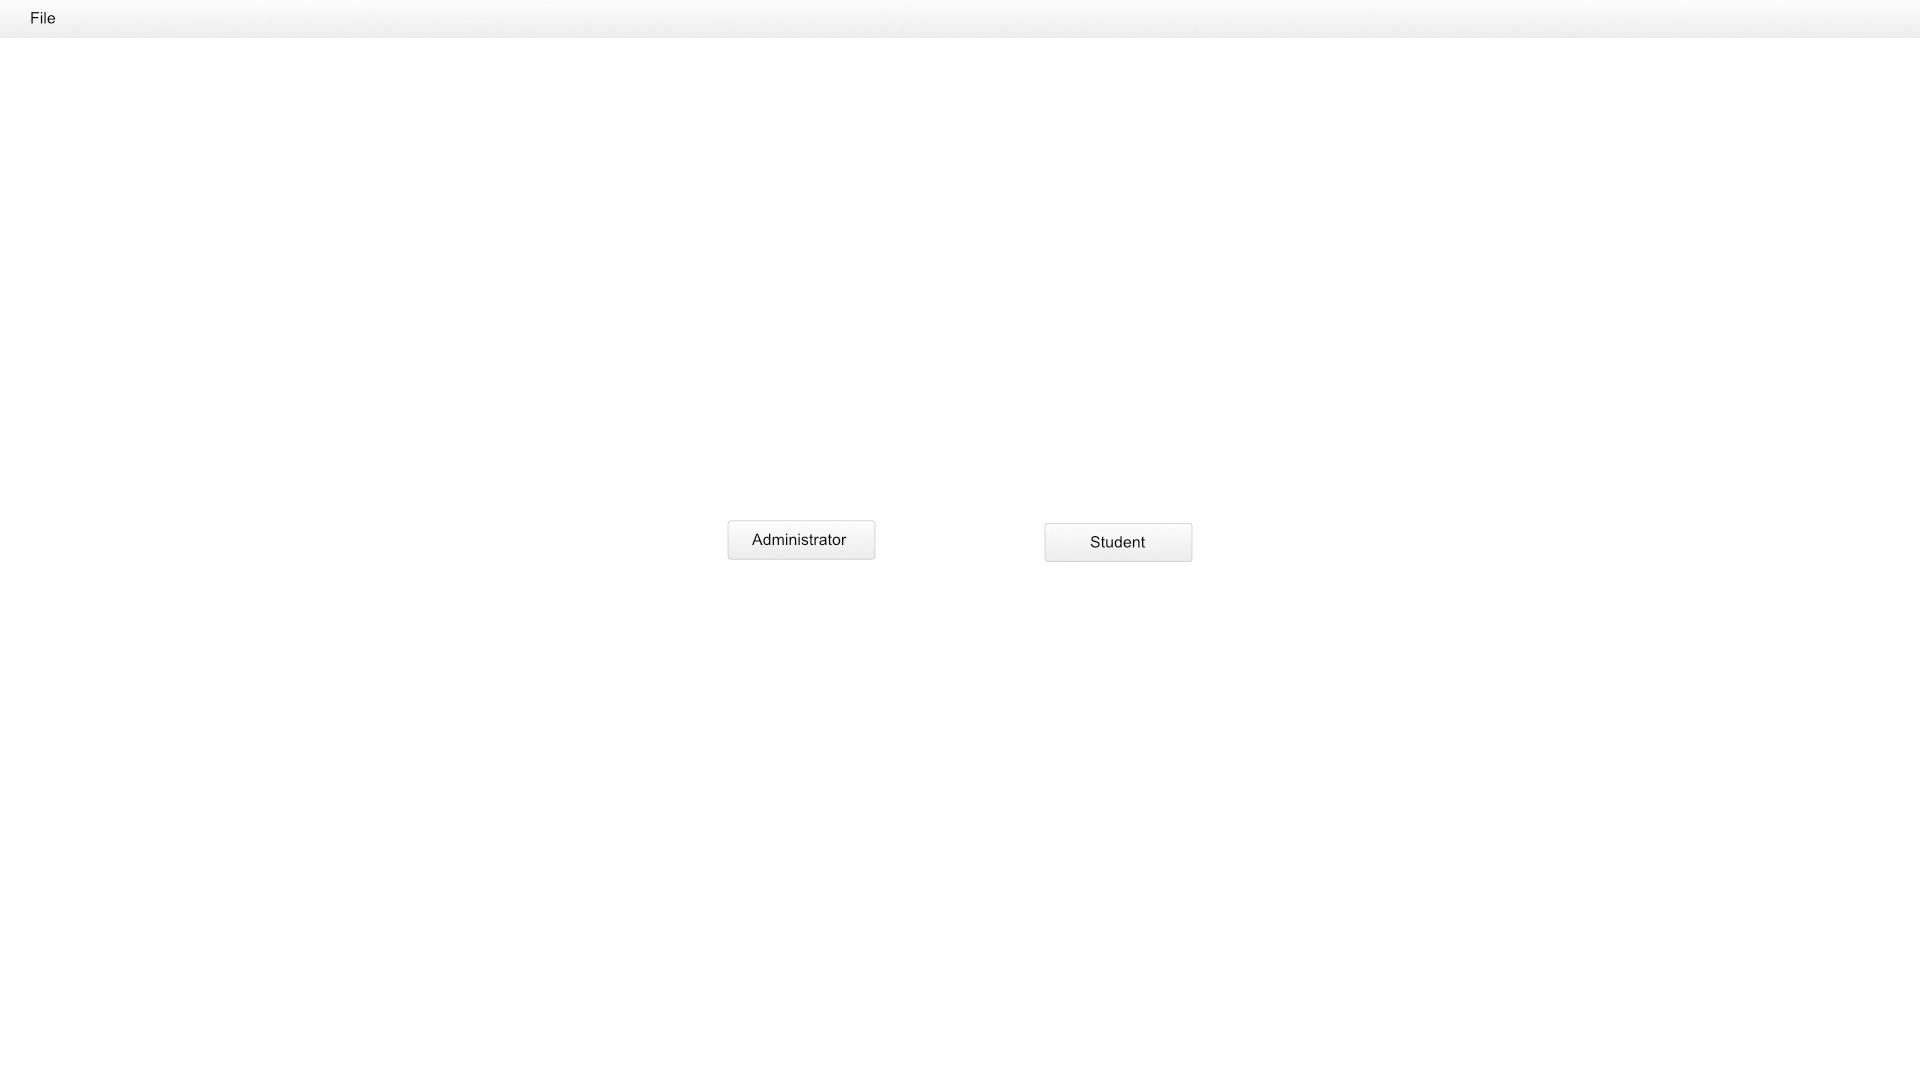
\includegraphics[width=\textwidth]{Bilder/Role-selection}
\\
\\
Dies ist das Startfenster der Anwendung. In diesem kann der Benutzer mit einem klick auf einen der angezeigten Buttons den Zugang auswählen welchen er nutzen möchte. Für die Benutzung der Anwendung als Student den Button \textit{Student} auswählen. Nach betätigen des Buttons lädt die Anwendung einige Sekunden bevor sich das nächste Fenster öffnet.


\subsection{Gruppenauswahl}
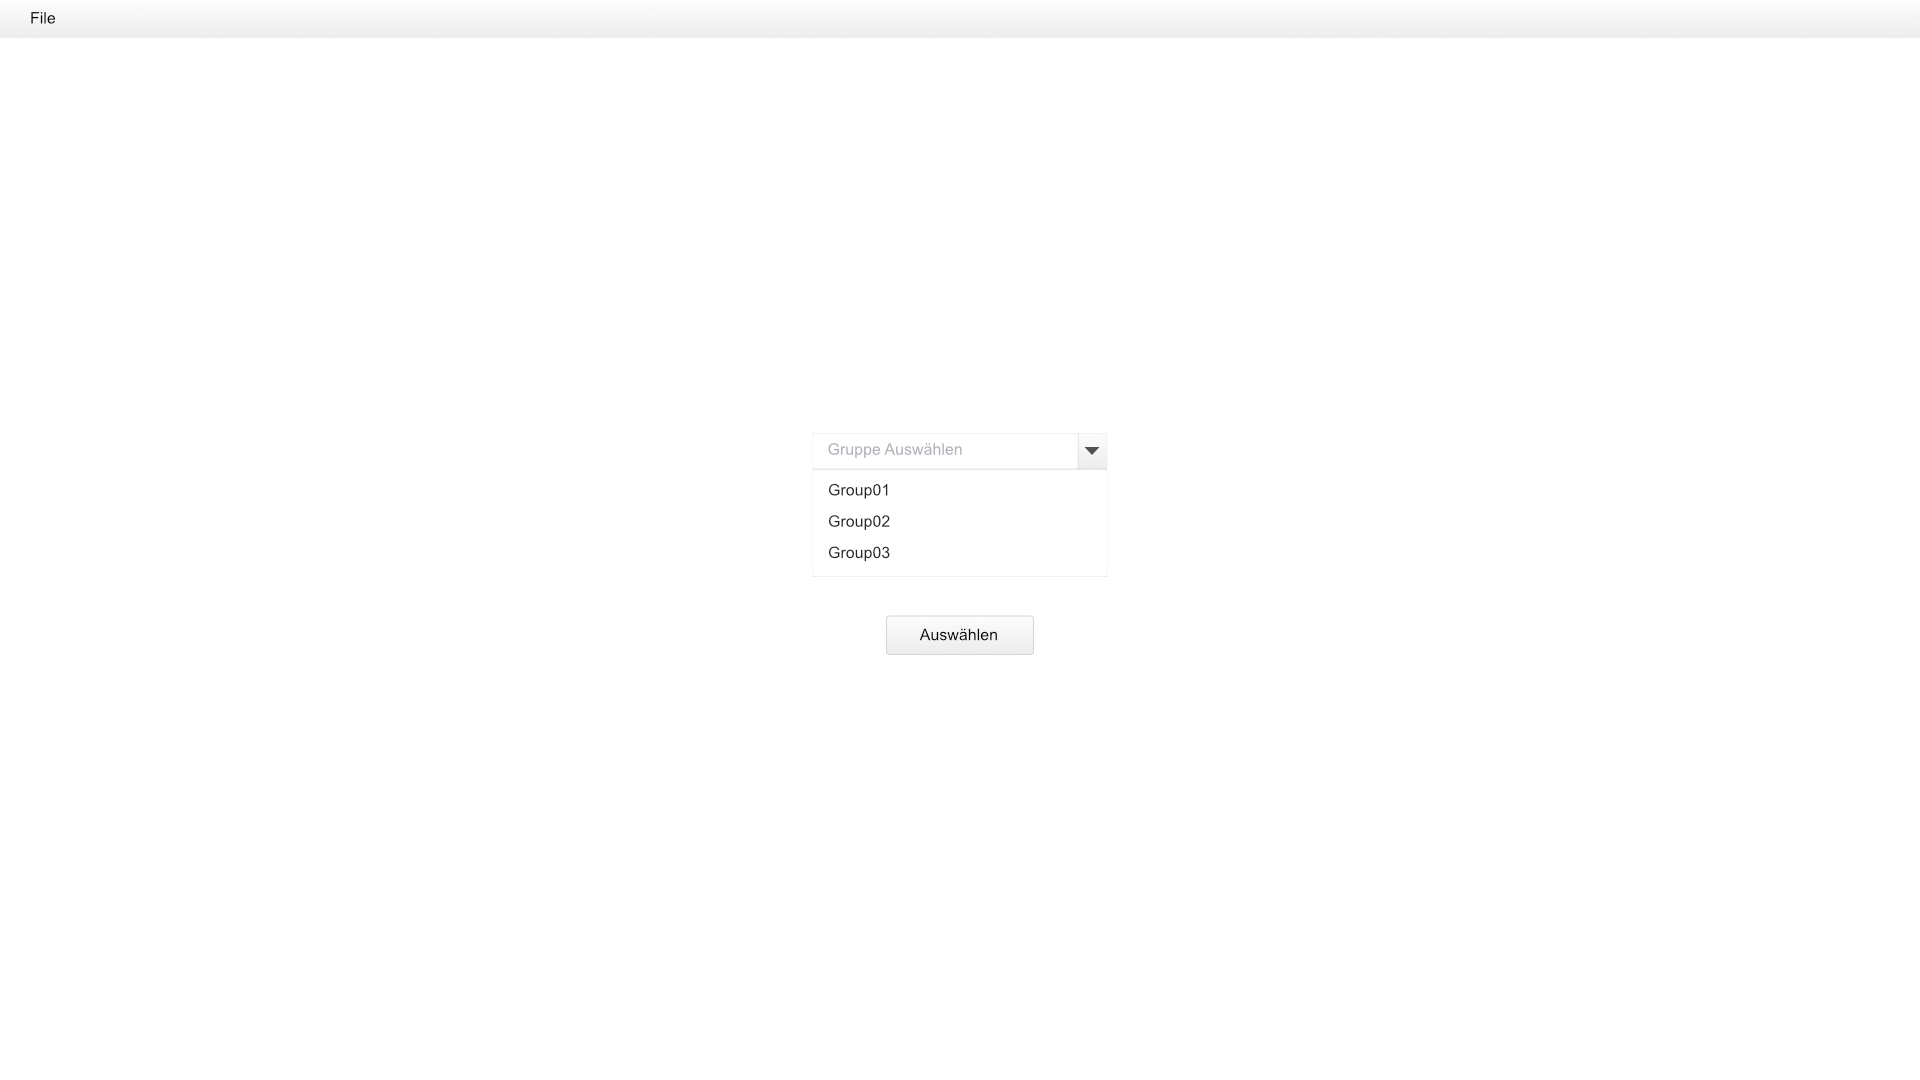
\includegraphics[width=\textwidth]{Bilder/Student/Group-selection}
\\
\\
Wurde die Rolle als Student ausgewählt öffnet sich das Fenster für die Gruppenauswahl. Die Gruppen sind entsprechend der Projekte nummeriert. Die Projektnummer ist in der Aufgabenstellung zu finden. 
\\
Die Gruppe wird mit einem klick auf den Namen ausgewählt und mit betätigen des Buttons \textit{Auswählen} öffnet sich die Terminübersicht.

\subsection{Übersicht}
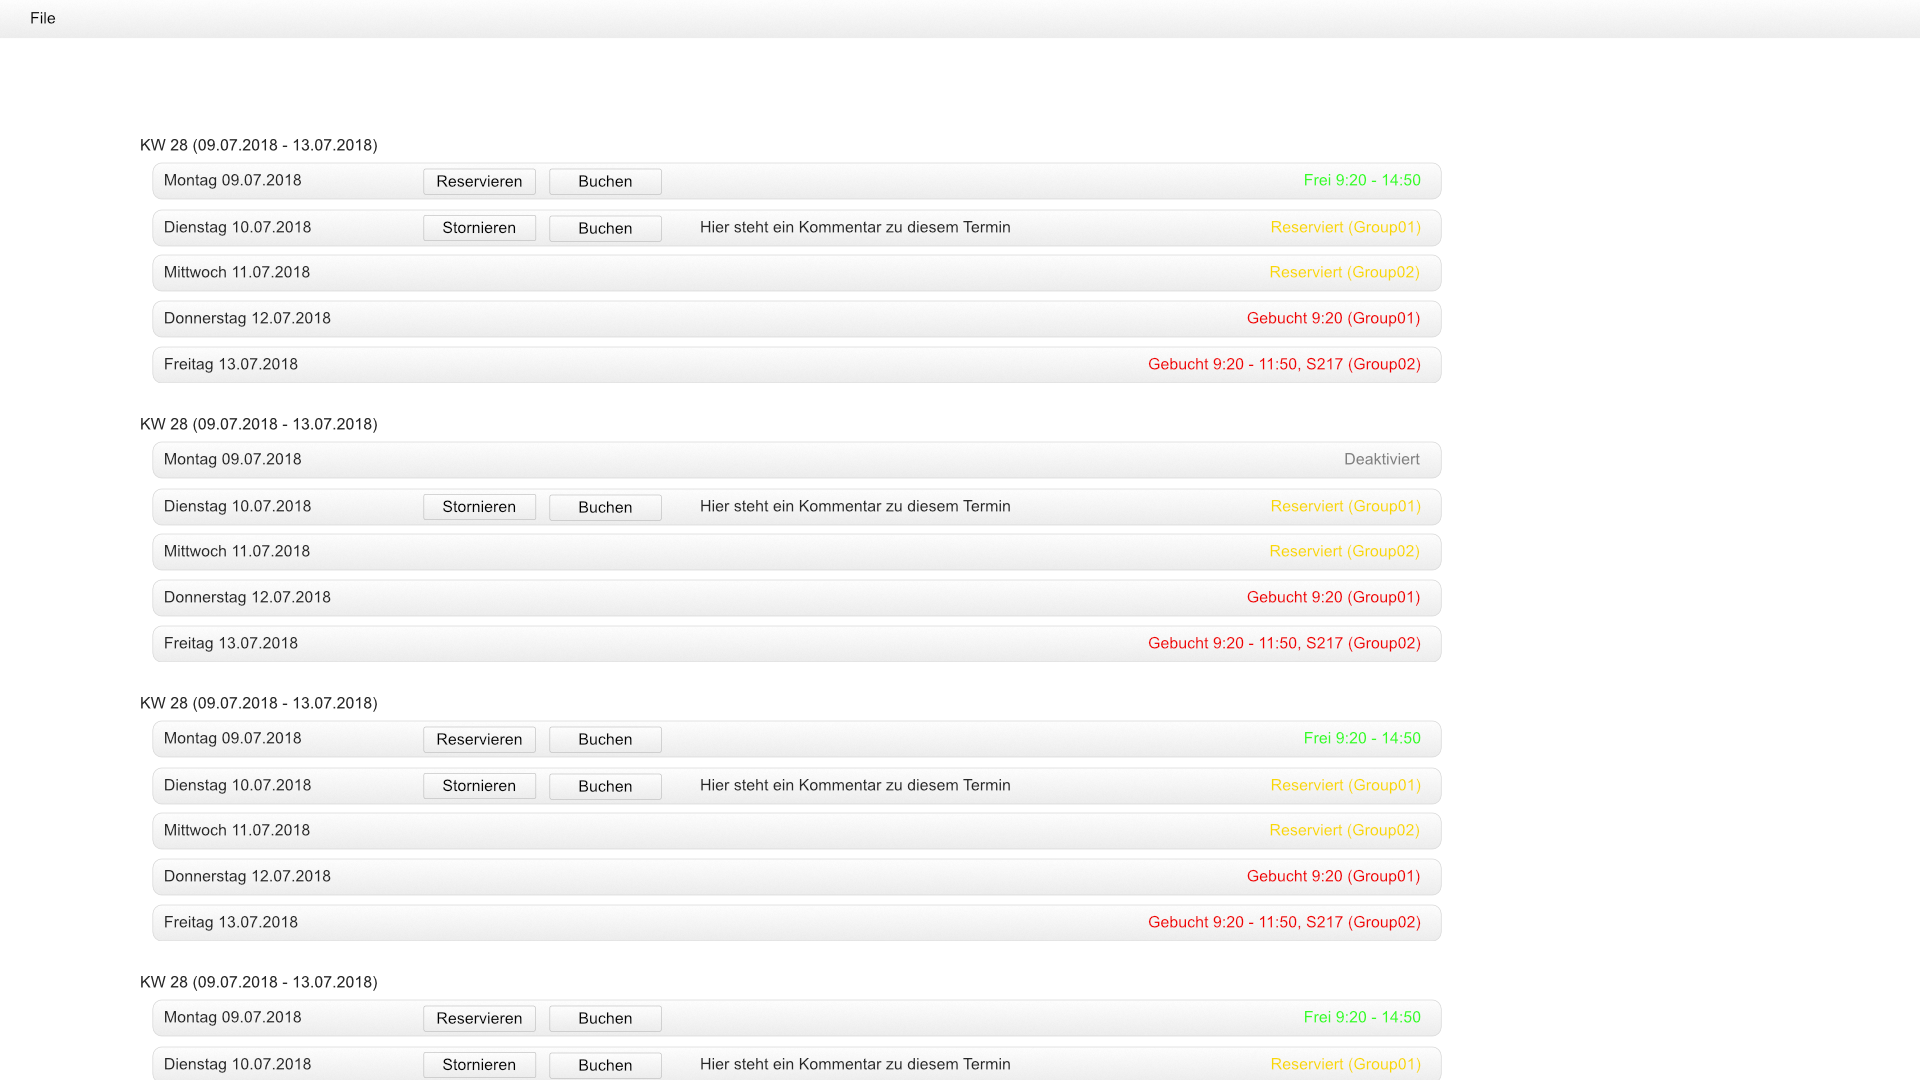
\includegraphics[width=\textwidth]{Bilder/Student/Date-management}
\\
\\
In der Terminübersicht können Tage mit dem Button \textit{Reservieren} reserviert und mit dem Button \textit{Buchen} gebucht werden. 
\\
Eine Reservierung belegt den kompletten Tag. Diese kann mit dem Button \textit{Stornieren} wieder entfernt werden oder mit den Button \textit{Buchen} in eine Buchung umgewandelt werden.

\subsubsection{Buchen}
\begin{wrapfigure}{R}{0.2\textwidth}
 	\centering
 	\includegraphics[width=0.4\textwidth]{Bilder/Buttons_clicked/Student-Book-Button-pressed}
\end{wrapfigure}
 Ist eine Buchung ausgewählt öffnet sich ein Fenster. In diesem kann die gewünschte Startzeit eingetragen und mit \textit{Buchen} bestätigt werden. 
 \\
 \\
 \textbf{Wichtig} ein Buchung ist fest und kann nur noch von dem Administrator geändert werden. Mehr als eine Buchung ist nicht möglich. 
